%\documentclass[12pt,a4paper]{report}
%\usepackage[utf8]{inputenc}
%\usepackage[english]{babel}
%\usepackage{amsmath}
%\usepackage{amsfonts}
%\usepackage{amssymb}
%\usepackage{graphicx}
%\usepackage{eurosym}
%\usepackage[left=2cm,right=2cm,top=2cm,bottom=2cm]{geometry}
%\usepackage{wrapfig}
%\usepackage{mathdots}
%\usepackage{caption}
%\usepackage{cite}
%\usepackage{mathrsfs}
%\usepackage{float}
%\author{Eva María Urbano González}
%\title{Data Link Layer Protocol}
%\begin{document}
%\maketitle
%\tableofcontents
%\listoffigures
%\listoftables
%\chapter{DLL}
\subsection{Functions of the DLL}
The Data-Link layer is the protocol layer in a program that handles the moving of data in and out across a physical link in a network. The Data-Link layer is layer 2 in the Open Systems Interconnect (OSI) model for a set of telecommunication protocols.
The DLL is responsible for converting data stream to signals bit by bit and to sent that over the underlying hardware.At the receiving end, DLL picks up data from hardware which are in the form of electrical signals, assembles them in a recognizable frame format, and hands over to upper layer. The DLL also ensures that an initial connection has been set up, divides output data into data frames, and handles the acknowledgements from a receiver that the data arrived successfully. It also ensures that incoming data has been received successfully by analyzing bit patterns at special places in the frames. The specific functions are the following ones\footnote{They are explaied in Annex II 7.1.1}.
\begin{itemize}
\item \textbf{Framing}
\item \textbf{Adressing}
\item \textbf{Synchronization}
\item \textbf{Flow control}
 \end{itemize}
\subsection{Working procedure}
The way these functions are achieved will be explained. To do so, a list of possible protocols from the simplest one to the more complex will briefly exposed. To see more information about these procedures as their algorithms and flow diagrams, Annex II 7.1.2 can be consulted. After knowing the main features of each one, a ranking of the prefered working procedures will be done. 
\subsubsection{Simplest Protocol}
\begin{itemize}
\item No error or flow control
\item Overwhelming is not considered
\item Only thing implemented: Request from adjacent layers.
\end{itemize}
\subsubsection{Stop-and-Wait Protocol}
Same features as the Simplest Protocol plus:
\begin{itemize}
\item Feedback from the receiver to the sender to manage overwhelming
\item ACK frames are used (simple tokens of acknowledgement) to tell the sender the receiver has receive the data and can continue sending frames.
\end{itemize}
\\
Simple Protocon and Stop-and-Wait Protocol can be suitable for noiseless channels. However, noiseless channels are nonexistent. There is a need to add error control to the protocol. Three protocols are discussed with the aim of doing so.
\subsubsection{Stop-and-Wait Automatic Repeat Request}
Same features as the Stop-and-Wait Protocol plus:
\begin{itemize}
\item Simple error control mechanism
\item Detection of corrupted frames
\item Detection of errors is manifested by the silence of the receiver
\item Timer exists in the sender. If time expires and there is no response (ACK) from the receiver, the frame is resent.
\item Innefficient system
\end{itemize}  
\subsubsection{Go-Back-N Automatic Repeat Request}
Improves the efficiency of the Stop-and-Wait Protocol with:
\begin{itemize}
\item Multiple frames in transition while waiting for achnowledgment.
\item ACK is sent if the frame is received without damage.
\item Detection of errors is manifested by the silence of the receiver
\item Sender resends all the frames beggining with the one from which no ACK has been received and its time is expired.
\end{itemize}
\subsubsection{Selective Repeat Automatic Repeat Request}
Improve the works at the sender-site but the work procedure at the receiver site is more complex.
\begin{itemize}
\item Allows frames to arrive out of order, the receiver orders them
\item ACK is sent when a frame has arrived satisfactory
\item NaK is sent if the frame has not arrived satisfactory
\item Sender only resends the corrupted or lost frame
\end{itemize}
\subsubsection{Bidirecional links: Piggybacking}
Piggybacking is not a protocol, is a technique. All que protocols explained until now are all unidirectional: data frames flow
in only one direction although control information such as ACK and NAK frames can
travel in the other direction. In real life, data frames are normally flowing in both directions:
from node A to node B and from node B to node A. This means that the control
information also needs to flow in both directions. Piggybacking is usedto improve the efficiency of the bidirectional protocols. When a frame is carrying
data from A to B, it can also carry control information about arrived (or lost) frames
from B; when a frame is carrying data from B to A, it can also carry control information
about the arrived (or lost) frames from A.
\subsubsection{Working procedure ranking}
Now its time to choose the working procedure that best fits the needs of the mission. To do so, an OWA (Ordered Weighted Average) will be used. The criteria to consider is the following one:
\begin{itemize}
\item Efficiency: This fact deals with how the channel is being used. Protocols will be classified as non-efficient or efficient. 
\item Time: This fact deals about the time needed to transmit the data satisfactory.
\item Error correction: Deals about whether a protocol can correct an error of transmission or not.
\end{itemize}
It is important also to take into account that the protocol to use should have a flow control, that is, should know if the receiver is available or not to receive the data. For this reason the Simplest Protocol is rejected and won't be studied in the OWA. Regarding the factors of the OWA, all of them will be rated from 0 to 1. In this project the fact of transmitting the data without errors is more important than transmitting it fast, as is possible to appreciate un the project charter ( the latency can be relative high, but incorrect information is useless). The efficiency of the protocol is very important too, because the less the efficiency the less power provided by the CubeSat is being used. Since the CubeSat has limited space, ideally al the power it can gives for transmittion will be used for it. Then, the weights of the different factors are the following ones:
\begin{itemize}
\item Efficiency: 40
\item Time: 30
\item Error correction: 60
\end{itemize} 
In the following table the rating of each protocol together with the corresponding OWA is shown. 
\begin{table}[H]
\begin{center}
\begin{tabular}{ | c | c | c | c | c |}
\hline
Protocol&Efficiency&Time&Error correction&OWA\\
\hline
Stop-and-Wait Protocol&0&0&0&0\\
\hline
Stop-and-Wait ARQ&0&0&1&0,46\\
\hline
Go-Back-N ARQ&1&0&1&0.69\\
\hline
Selective Repeat ARQ&1&1&1&1\\
\hline
\end{tabular}
\caption{OWA of the DLL protocols.}
\end{center}
\end{table} 
Then, the ranking of working procedures is the following one: 
\begin{table}[H]
\begin{center}
\begin{tabular}{|c|c|}
\hline
\textbf{1}&Selective Repeat ARQ\\
\hline
\textbf{2}&Go-Back-N ARQ\\
\hline
\textbf{3}&Stop-and-Wait ARQ\\
\hline
\textbf{4}&Stop-and-Wait Protocol\\
\hline
\end{tabular}
\caption{Ranking of working procedures}
\end{center}
\end{table}
It has to be said that when dealing with bidirecional links piggybacking technique will be used if possible.
\subsection{Protocols}
The standards of the CCSDS will be followed in order to allow interoperability with other satellites such as the one of the client. The CCSDS has developed four protocols for the Data Link Protocol Sublayer of the Data Link Layer\cite{Secretariat2014}:
\begin{itemize}
\item TM Space Data Link Protocol
\item TC Space Data Link Protocol
\item AOS Space Data Link Protocol
\item Proximity-1 Space Link Protocol-Data Link Layer
\end{itemize}
These protocols provide the capability to send data over a single space link. TM, TC, and AOS can have secured user data into a frame using the Space Data Link Security (SDLS) Protocol.\\
 CCSDS has also developed three standards for the Synchronization and Channel Coding Sublayer of the DLL:
 \begin{itemize}
 \item TM Synchronization and Channel Coding
 \item TC Synchronization and Channel Coding
 \item Proximity-1 Space Link Protocol—Coding and Synchronization Layer
 \end{itemize}
TM Synchronization and Channel Coding is used with the TM or AOS Space Data Link
Protocol, TC Synchronization and Channel Coding is used with the TC Space Data Link Protocol and the Proximity-1 Space Link Protocol—Coding and Synchronization Layer is
used with the Proximity-1 Space Link Protocol—Data Link Layer. This can be seen better in the following image.\\
\begin{figure}[H]
\begin{center}
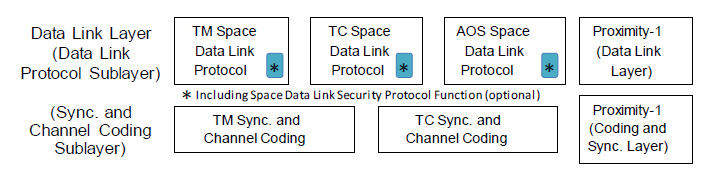
\includegraphics[scale=0.9]{DLLCCSDS.PNG}   
\caption{DLL of the CCSDS.}
\end{center}
\end{figure}
Now the reliability of each of the protocols of the Data Link Protocol Sublayer will be compared in order to know which one is the best of them. This will be done because reliability is the most important feature of the DLL.
\begin{table}[H]
\begin{center}
\begin{tabular}{|c|c|}
\hline
\textbf{Protocol}&\textbf{System used for reliability}\\
\hline
TM&Stop-and-Wait Protocol\\
\hline
TC&Type-A: Go-Back-N ARQ, Type-B:Stop-and-Wait Protocol\\
\hline
AOS&Stop-and-Wait Protocol\\
\hline
Proximity-1&Go-Back-N ARQ\\
\hline
\end{tabular}
\caption{Reliability of CCSDS protocols}
\end{center}
\end{table}
According to the table and to the ranking of working procedures done previously, only TC Type-A and Proximity-1 will be considered from now on. Security is another important feature to take into account when taking this decision. TM Space Data Link Protocol has provision for inserting secured data into a frame using the Space Data Link Security (SDLS) Protocol. However, there have been no security requirements to date established for Proximity-1. The SLDS protocol can provide security services, such as authentication and confidentiality for TC Transfer Frames (it can also do it with TM and AOS, that have been previously discharted). Both the TC and the Proximity-1 use variable-lenght Transfer Frames to facilitate reception of short messages with short delay. Another key feature to take into account when deciding a protocol, is the concept of "Virtual Channels". The
Virtual Channel facility allows one Physical Channel (a stream of bits transferred over a
space link in a single direction) to be shared among multiple higher-layer data streams, each
of which may have different service requirements. A single Physical Channel may therefore
be divided into several separate logical data channels, each known as a Virtual Channel
(VC). The TC has the following identifiers: the Transfer Frame Version Number (TFVN), the Spacecraft Identifier (SCID), and the Virtual Channel Identifier (VCID). It also uses an optional identifier, called the Multiplexer Access Point Identifier (MAP ID), that is used to create multiple streams of data within a Virtual Channel. In contrast, the Proximity-1 uses a triad of multiplexing capabilities, which is incorporated for specific funcionality within the link. The Spacecraft Identifier (SCID) identifies the source or destination of Transfer Frames transported in the link connection based upon the Source-or-Destination Identifier. The Pysical Channel Identifier (PCID) provides up to two independently multiplexed channels. The Port ID provides the means to route user data internally to specific logic ports, such as applications or transport processes, or to physical ports, such as onboard buses or physical connections. Now a table with the identifiers of the TC and the Proximity-1 will be shown:
\begin{table}[H]
\begin{center}
\begin{tabular}{|c|c|c|}
\hline
Identifiers&TC Space Data Link Protocol&Proximity-1 Space Link Protocol- Data Link Layer\\
\hline
TFVN&00&10\\
\hline
SCID&0 to 1023&0 to 2013\\
\hline
PCID&N/A&0 to 1\\
\hline
VCID&0 to 63&N/A\\
\hline
MAP ID&0 to 63&N/A\\
\hline
Port identifier&N/A&0 to 7\\
\hline
\end{tabular}
\caption{Identifiers of TC and Proximity-1 Space Data Link Layer Protocols}
\end{center}
\end{table} 
Having Virtual Channels is important for the mission that is exposed in this project because it allows having more than one stream of bits to take place at the same time, that is to say that more than one client can communicate with their satellite without having to wait for another client to finish.\\
The decision taken is to use the TC Space Data Link Protocol with the TC sync. and channel coding together with the Space Data Link Security Protocol. The reasons for doing so are mainly:
\begin{itemize}
\item Security: Incorporing the SLDS authentication and confidentality is provided.
\item More virtual channels: This feature allow more clients communicating with their satellites at the same time.
\end{itemize}
More information about the chosen protocols such as the amount of bits occupied by the header, its configuration and total lenght can be found at Annex II 7.1.3 and Annex II 7.1.4.

%\bibliographystyle{unsrt}
%\bibliography{forouzan,Secretariat2014,TC,tmsynch} 
%\end{document}